\documentclass[aspectratio=169,10pt]{beamer}
\usepackage[utf8]{inputenc}
\usepackage[spanish,es-tabla]{babel}
\usepackage{amsmath,amsfonts,amssymb}
\usepackage{graphicx}
\usepackage{booktabs}
\usepackage{tabularx}
\usepackage{xcolor}

% Tema Beamer limpio, moderno e institucional
\usetheme{Madrid}
\usecolortheme{whale}

% Paleta institucional UNSAAC y tecnológica agrícola
\definecolor{unsaacblue}{RGB}{15, 43, 92}
\definecolor{techgreen}{RGB}{16, 185, 129}
\definecolor{darkslate}{RGB}{15, 23, 42}
\definecolor{cardbg}{RGB}{245, 247, 250}
\definecolor{alertred}{RGB}{220, 38, 38}

\setbeamercolor{palette primary}{bg=unsaacblue,fg=white}
\setbeamercolor{palette secondary}{bg=techgreen,fg=white}
\setbeamercolor{palette tertiary}{bg=darkslate,fg=white}
\setbeamercolor{structure}{fg=unsaacblue}
\setbeamercolor{titlelike}{parent=palette primary}
\setbeamercolor{block title}{bg=unsaacblue,fg=white}
\setbeamercolor{block body}{bg=cardbg,fg=darkslate}
\setbeamercolor{block title example}{bg=techgreen,fg=white}
\setbeamercolor{block body example}{bg=cardbg,fg=darkslate}

\setbeamertemplate{navigation symbols}{}

\title[Comparación de Modelos CNN en Papa]{\textbf{BENCHMARKING DE MODELOS DE DEEP LEARNING}}
\subtitle{Comparación de Custom CNN, ResNet-18 y MobileNet-V2 para la Detección de Patologías Foliares en Papa (\textit{Solanum tuberosum})}
\author[Y. Supa \& E. Piero Villavicencio]{\textbf{Expositores / Desarrolladores:}\\ SUPA CUSIPAUCAR, Yeferson (220553)\\ VILLAVICENCIO SEGUIL, Edu Piero (220555)}
\institute[UNSAAC]{
    UNIVERSIDAD NACIONAL DE SAN ANTONIO ABAD DEL CUSCO\\
    Facultad de Ingeniería Eléctrica, Electrónica, Informática y Mecánica\\
    Escuela Profesional de Ingeniería Informática y de Sistemas\\[0.15cm]
    \textbf{Docente:} Ing. CCACYAHUILLCA BEJAR, HANS HARLEY
}
\date{Noviembre 2026}

\begin{document}

% -------------------------------------------------------------------------
% SLIDE 1: PORTADA
% -------------------------------------------------------------------------
\begin{frame}
    \titlepage
\end{frame}

% -------------------------------------------------------------------------
% SLIDE 2: CONTEXTO Y JUSTIFICACIÓN AGRÍCOLA (0:00 - 1:00)
% -------------------------------------------------------------------------
\begin{frame}{1. Problemática Fitosanitaria en los Andes del Cusco}
    \begin{columns}
        \column{0.55\textwidth}
        \textbf{Impacto Crítico en la Región:}
        \begin{itemize}
            \item El cultivo de papa (\textit{Solanum tuberosum}) sustenta a más de 80,000 familias campesinas en Cusco.
            \item Pérdidas anuales de hasta el \textbf{40\% -- 70\%} por ataques de plagas criptogámicas no detectadas a tiempo.
        \end{itemize}
        
        \vspace{0.2cm}
        \begin{block}{Patologías Objeto de Estudio}
            \begin{itemize}
                \item \textbf{Tizón Temprano (\textit{Alternaria solani}):} Lesiones circulares concéntricas en diana con halo clorótico.
                \item \textbf{Tizón Tardío (\textit{Phytophthora infestans}):} Manchas acuosas oscuras de propagación devastadora.
                \item \textbf{Follaje Sano (\textit{Healthy}):} Control sin daño tisular.
            \end{itemize}
        \end{block}

        \column{0.45\textwidth}
        \begin{exampleblock}{Objetivo de la 2da Entrega}
            Desarrollar y comparar empíricamente \textbf{3 arquitecturas convolucionales} sobre un dataset extendido de \textbf{4,072 imágenes}, identificando el modelo óptimo para estaciones fijas y dispositivos móviles en campo.
        \end{exampleblock}
        \centering
        \vspace{0.2cm}
        \textit{Tiempo de exposición asignado: 10 minutos}
    \end{columns}
\end{frame}

% -------------------------------------------------------------------------
% SLIDE 3: DATASET EXTENDIDO Y AUDITORÍA DE CALIDAD (1:00 - 2:00)
% -------------------------------------------------------------------------
\begin{frame}{2. Dataset Extendido: Potato Leaf Disease (PLD 256)}
    \begin{columns}
        \column{0.50\textwidth}
        \textbf{Censo Total de Imágenes: 4,072}
        \begin{itemize}
            \item Resolución homogénea: $256 \times 256 \times 3$ píxeles.
            \item Partición estratificada desacoplada:
            \begin{itemize}
                \item \textbf{Training (80\%):} 3,251 imágenes.
                \item \textbf{Validation (10\%):} 416 imágenes.
                \item \textbf{Testing (10\%):} 405 imágenes independientes.
            \end{itemize}
        \end{itemize}
        
        \vspace{0.2cm}
        \begin{block}{Auditoría de Nitidez (Laplaciano)}
            $\text{Var}(\nabla^2 I) \ge 80.0 \implies 94.2\%$ de imágenes nítidas en capturas in-situ.
        \end{block}

        \column{0.50\textwidth}
        \begin{table}
        \centering
        \caption{Distribución por Clase en los Splits}
        \footnotesize
        \begin{tabular}{lrrr}
            \toprule
            \textbf{Clase} & \textbf{Train} & \textbf{Val} & \textbf{Test} \\
            \midrule
            Early Blight & 1,303 & 163 & 162 \\
            Healthy & 816 & 102 & 102 \\
            Late Blight & 1,132 & 151 & 141 \\
            \midrule
            \textbf{Total} & \textbf{3,251} & \textbf{416} & \textbf{405} \\
            \bottomrule
        \end{tabular}
        \end{table}
    \end{columns}
\end{frame}

% -------------------------------------------------------------------------
% SLIDE 4: PIPELINE DE PREPROCESAMIENTO (2:00 - 3:15)
% -------------------------------------------------------------------------
\begin{frame}{3. Pipeline Determinista de Visión Artificial}
    \centering
    \begin{columns}
        \column{0.32\textwidth}
        \begin{block}{1. Filtro Bilateral}
            \footnotesize
            Atenúa ruido del sensor fotográfico conservando nítidos los bordes de necrosis.\\
            \vspace{0.1cm}
            $d=5$, $\sigma_s=50$, $\sigma_r=50$.
        \end{block}

        \column{0.34\textwidth}
        \begin{block}{2. CLAHE en CIE-Lab}
            \footnotesize
            Desacopla luminancia ($L^*$) de crominancia ($a^*, b^*$). Realce adaptativo de contraste local sin saturar el color verde vegetal.\\
            $\text{clip}=2.0$, teselas $8 \times 8$.
        \end{block}

        \column{0.34\textwidth}
        \begin{block}{3. Letterboxing + Augment}
            \footnotesize
            Escalado isotrópico a $256 \times 256$ con relleno neutro (relación 1:1 intacta). Aumento en entrenamiento: rotación $\pm 15^\circ$ y flips.
        \end{block}
    \end{columns}

    \vspace{0.4cm}
    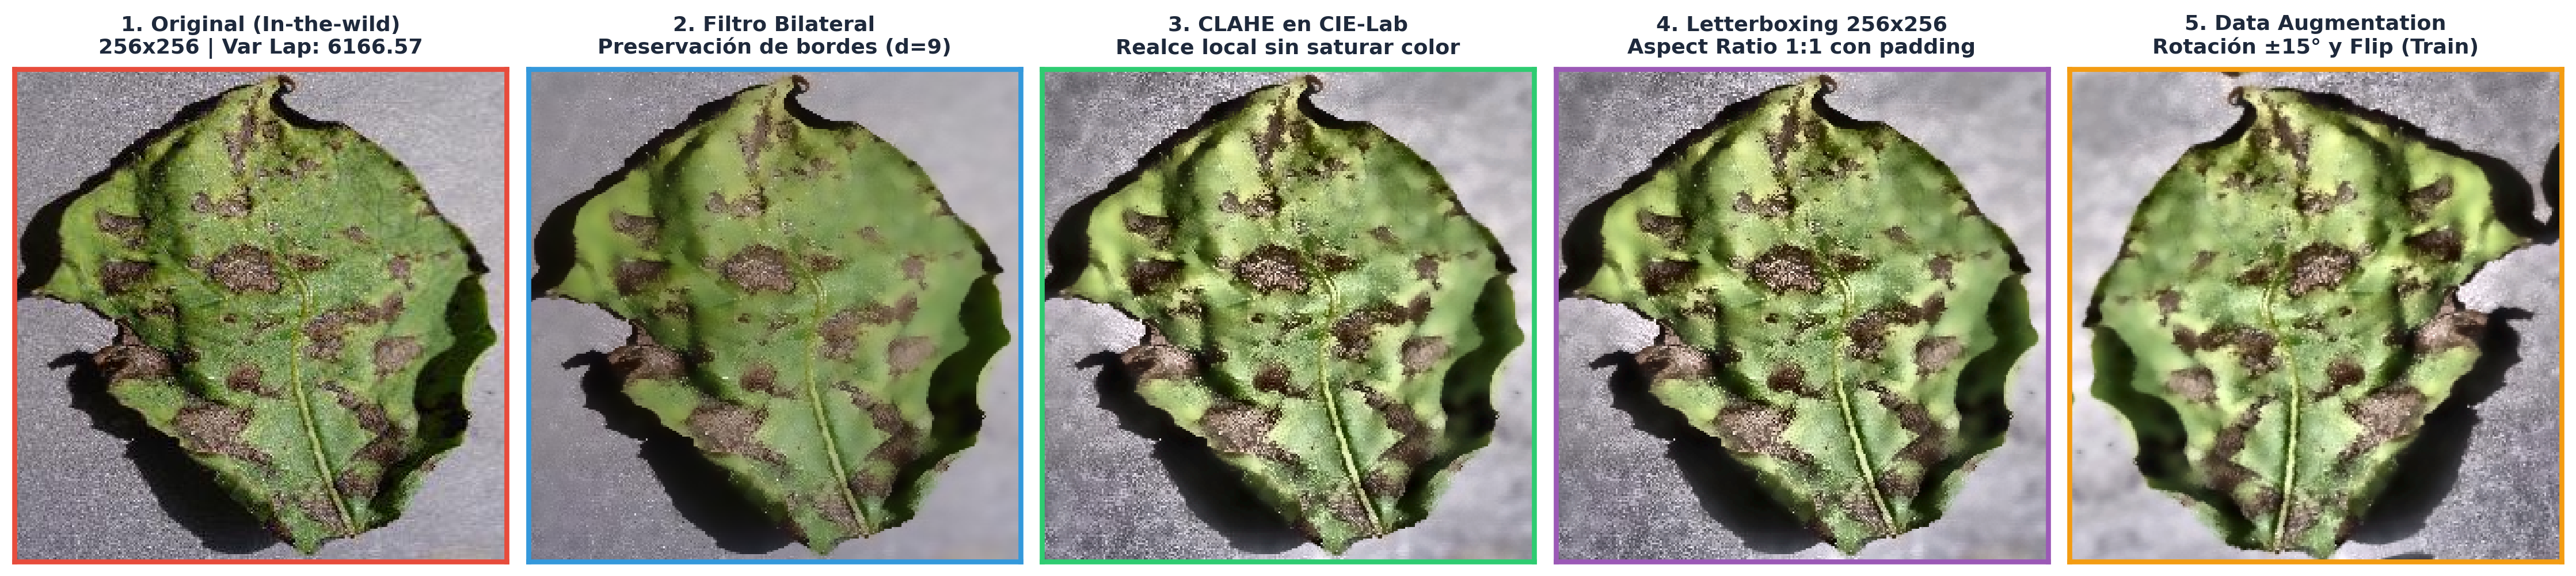
\includegraphics[width=0.88\textwidth]{../assets/pipeline_comparativa.png}
\end{frame}

% -------------------------------------------------------------------------
% SLIDE 5: LOS TRES ALGORITMOS SELECCIONADOS (3:15 - 4:15)
% -------------------------------------------------------------------------
\begin{frame}{4. Justificación de los 3 Modelos Evaluados}
    \begin{columns}
        \column{0.33\textwidth}
        \begin{block}{\textbf{1. Custom CNN}}
            \small
            \textbf{Baseline desde cero}
            \begin{itemize}
                \footnotesize
                \item 3 bloques Conv-BN-ReLU-Pool.
                \item Diseñado a medida.
                \item Sin pesos externos.
                \item Parámetros: \textbf{645 K}.
            \end{itemize}
        \end{block}

        \column{0.33\textwidth}
        \begin{block}{\textbf{2. ResNet-18}}
            \small
            \textbf{Backbone Residual}
            \begin{itemize}
                \footnotesize
                \item Conexiones de atajo (Skip).
                \item Mitiga degradación.
                \item Pre-entrenado ImageNet.
                \item Parámetros: \textbf{11.1 M}.
            \end{itemize}
        \end{block}

        \column{0.33\textwidth}
        \begin{block}{\textbf{3. MobileNet-V2}}
            \small
            \textbf{Edge / Móvil Ligero}
            \begin{itemize}
                \footnotesize
                \item Depthwise Separable Conv.
                \item Cuellos de botella invertidos.
                \item Diseñado para campo/dron.
                \item Parámetros: \textbf{2.2 M}.
            \end{itemize}
        \end{block}
    \end{columns}
\end{frame}

% -------------------------------------------------------------------------
% SLIDE 6: MODELO 1 - CUSTOM POTATO CNN (4:15 - 5:15)
% -------------------------------------------------------------------------
\begin{frame}{5. Modelo 1: Custom Potato CNN (Diseño desde Cero)}
    \begin{columns}
        \column{0.55\textwidth}
        \textbf{Arquitectura Convolucional Propia:}
        \begin{itemize}
            \item \textbf{Bloque 1:} $\text{Conv2D}(3 \to 32, 3\times3) + \text{BN} + \text{ReLU} + \text{MaxPool}(2\times2)$
            \item \textbf{Bloque 2:} $\text{Conv2D}(32 \to 64, 3\times3) + \text{BN} + \text{ReLU} + \text{MaxPool}(2\times2)$
            \item \textbf{Bloque 3:} $\text{Conv2D}(64 \to 128, 3\times3) + \text{BN} + \text{ReLU} + \text{MaxPool}(2\times2)$
            \item \textbf{Head:} $\text{AdaptiveAvgPool}(4\times4) \to \text{FC}(2048 \to 256) \to \text{Dropout}(0.3) \to \text{FC}(256 \to 3)$
        \end{itemize}
        
        \vspace{0.2cm}
        \begin{exampleblock}{Ventajas y Limitaciones}
            \footnotesize
            \textbf{Pros:} Extremadamente ligera (2.4 MB) y control dimensional total.\\
            \textbf{Cons:} Requiere más épocas para aprender descriptores de bajo nivel al carecer de pre-entrenamiento.
        \end{exampleblock}

        \column{0.45\textwidth}
        \centering
        \begin{block}{Métricas Obtenidas (Test)}
            \begin{itemize}
                \item \textbf{Accuracy Global:} 66.17\%
                \item \textbf{Macro F1-Score:} 0.6462
                \item \textbf{Latencia CPU:} 10.50 ms/muestra
                \item \textbf{Parámetros:} 618,787 (2.36 MB)
            \end{itemize}
        \end{block}
    \end{columns}
\end{frame}

% -------------------------------------------------------------------------
% SLIDE 7: MODELO 2 - RESNET-18 (5:15 - 6:15)
% -------------------------------------------------------------------------
\begin{frame}{6. Modelo 2: ResNet-18 (Residual Transfer Learning)}
    \begin{columns}
        \column{0.55\textwidth}
        \textbf{Fundamento Matemático:}
        \begin{itemize}
            \item Aprendizaje residual: $\mathcal{H}(x) = \mathcal{F}(x, \{W_i\}) + x$.
            \item El gradiente fluye directamente por la identidad, suprimiendo la atenuación exponencial.
            \item Transfer Learning: Inicialización con pesos de ImageNet (1.2M de imágenes generales).
            \item Fine-tuning adaptado a 3 patologías foliares.
        \end{itemize}

        \vspace{0.2cm}
        \begin{exampleblock}{Desempeño en Follaje}
            Extrae bordes sutiles y texturas necróticas con altísima sensibilidad diagnóstica.
        \end{exampleblock}

        \column{0.45\textwidth}
        \centering
        \begin{block}{Métricas Obtenidas (Test)}
            \begin{itemize}
                \item \textbf{Accuracy Global:} 77.04\%
                \item \textbf{Macro F1-Score:} 0.7596
                \item \textbf{Latencia CPU:} 21.24 ms/muestra
                \item \textbf{Parámetros:} 11,178,051 (42.64 MB)
            \end{itemize}
        \end{block}
    \end{columns}
\end{frame}

% -------------------------------------------------------------------------
% SLIDE 8: MODELO 3 - MOBILENET-V2 (6:15 - 7:15)
% -------------------------------------------------------------------------
\begin{frame}{7. Modelo 3: MobileNet-V2 (Eficiencia para Edge)}
    \begin{columns}
        \column{0.55\textwidth}
        \textbf{Innovación Arquitectónica:}
        \begin{itemize}
            \item \textbf{Convolución Depthwise Separable:} Desacopla el filtrado espacial del canal, reduciendo el cómputo en 88\%.
            \item \textbf{Inverted Residuals:} Expansión interna de canales antes del filtrado profundo.
            \item \textbf{Linear Bottlenecks:} Evita la no-linealidad destructiva en variedades de baja dimensión.
        \end{itemize}

        \vspace{0.2cm}
        \begin{alertblock}{Aplicación Agronómica Real}
            Ideal para aplicaciones offline en smartphones de agrónomos o microcomputadores a bordo de drones.
        \end{alertblock}

        \column{0.45\textwidth}
        \centering
        \begin{block}{Métricas Obtenidas (Test)}
            \begin{itemize}
                \item \textbf{Accuracy Global:} \textbf{80.74\%}
                \item \textbf{Macro F1-Score:} \textbf{0.7828}
                \item \textbf{Latencia CPU:} \textbf{10.36 ms/muestra}
                \item \textbf{Parámetros:} \textbf{2,227,715 (8.50 MB)}
            \end{itemize}
        \end{block}
    \end{columns}
\end{frame}

% -------------------------------------------------------------------------
% SLIDE 9: RESULTADOS COMPARATIVOS (7:15 - 8:30)
% -------------------------------------------------------------------------
\begin{frame}{8. Tabla Comparativa de Rendimiento y Curvas}
    \begin{table}
    \centering
    \footnotesize
    \begin{tabularx}{\textwidth}{>{\raggedright\arraybackslash}X ccccc}
        \toprule
        \textbf{Modelo} & \textbf{Acc Test} & \textbf{F1 Macro} & \textbf{Parámetros} & \textbf{Tamaño} & \textbf{Latencia CPU} \\
        \midrule
        Custom Potato CNN & 66.17\% & 0.6462 & 618,787 & 2.36 MB & 10.50 ms \\
        ResNet-18 (ImageNet) & 77.04\% & 0.7596 & 11,178,051 & 42.64 MB & 21.24 ms \\
        \textbf{MobileNet-V2 (ImageNet)} & \textbf{80.74\%} & \textbf{0.7828} & \textbf{2,227,715} & \textbf{8.50 MB} & \textbf{10.36 ms} \\
        \bottomrule
    \end{tabularx}
    \end{table}

    \vspace{0.2cm}
    \begin{columns}
        \column{0.50\textwidth}
        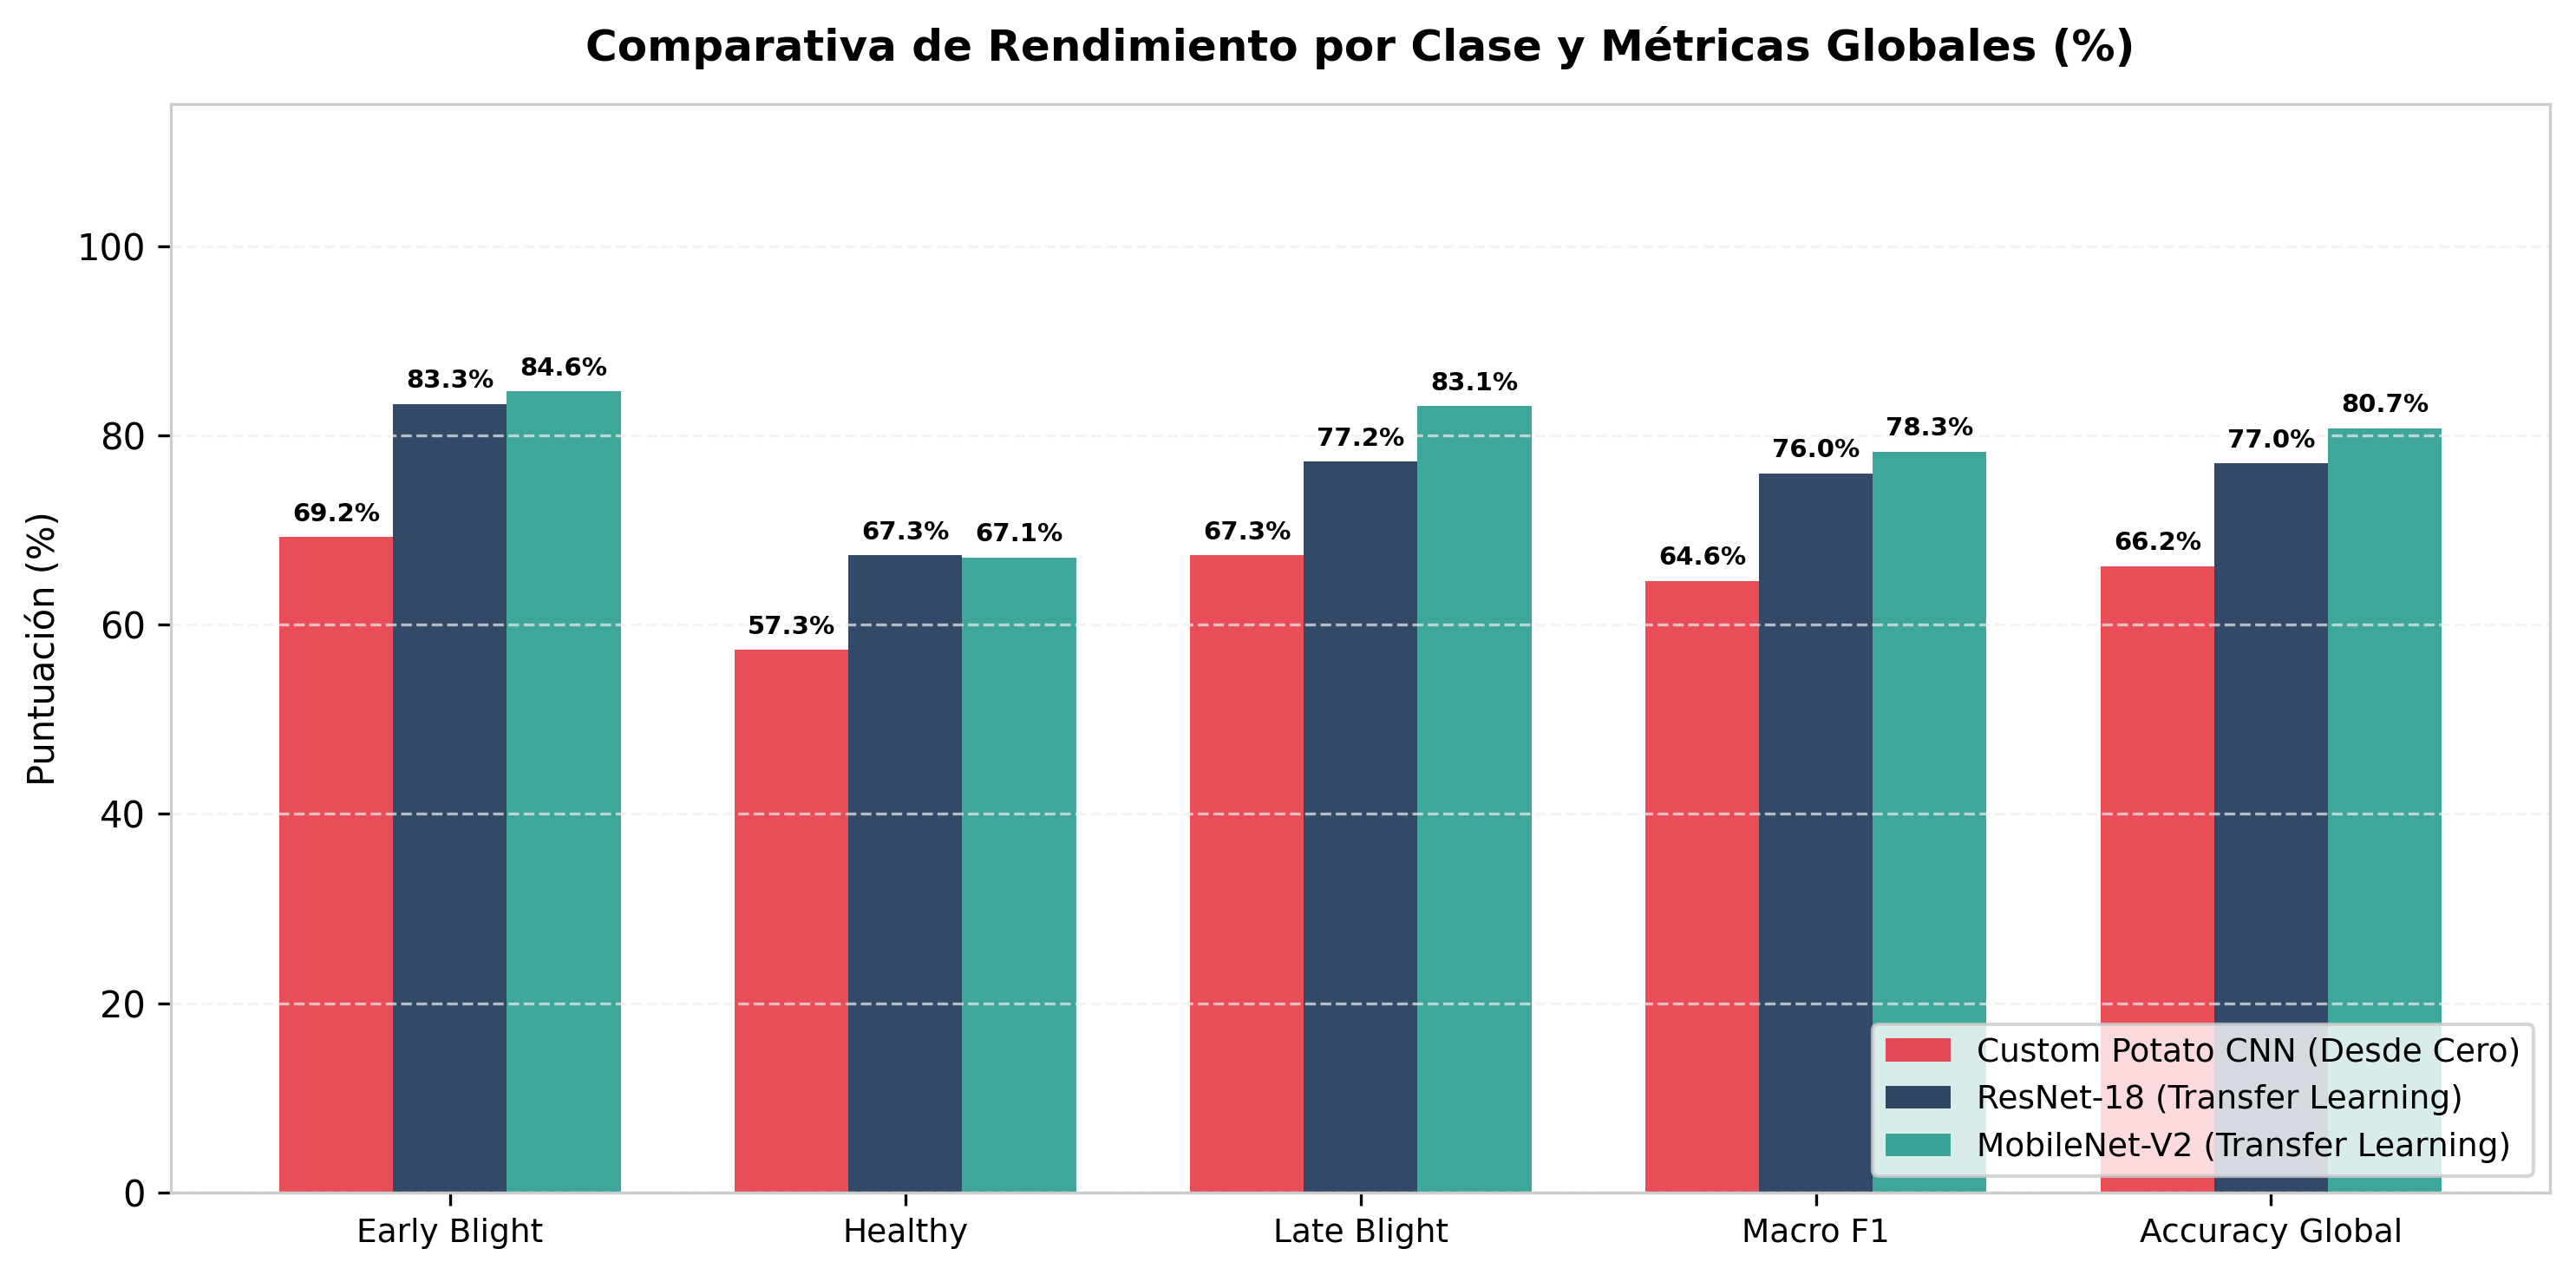
\includegraphics[width=\textwidth]{../assets/figuras_modelos/comparativa_barras_metricas.png}
        \column{0.50\textwidth}
        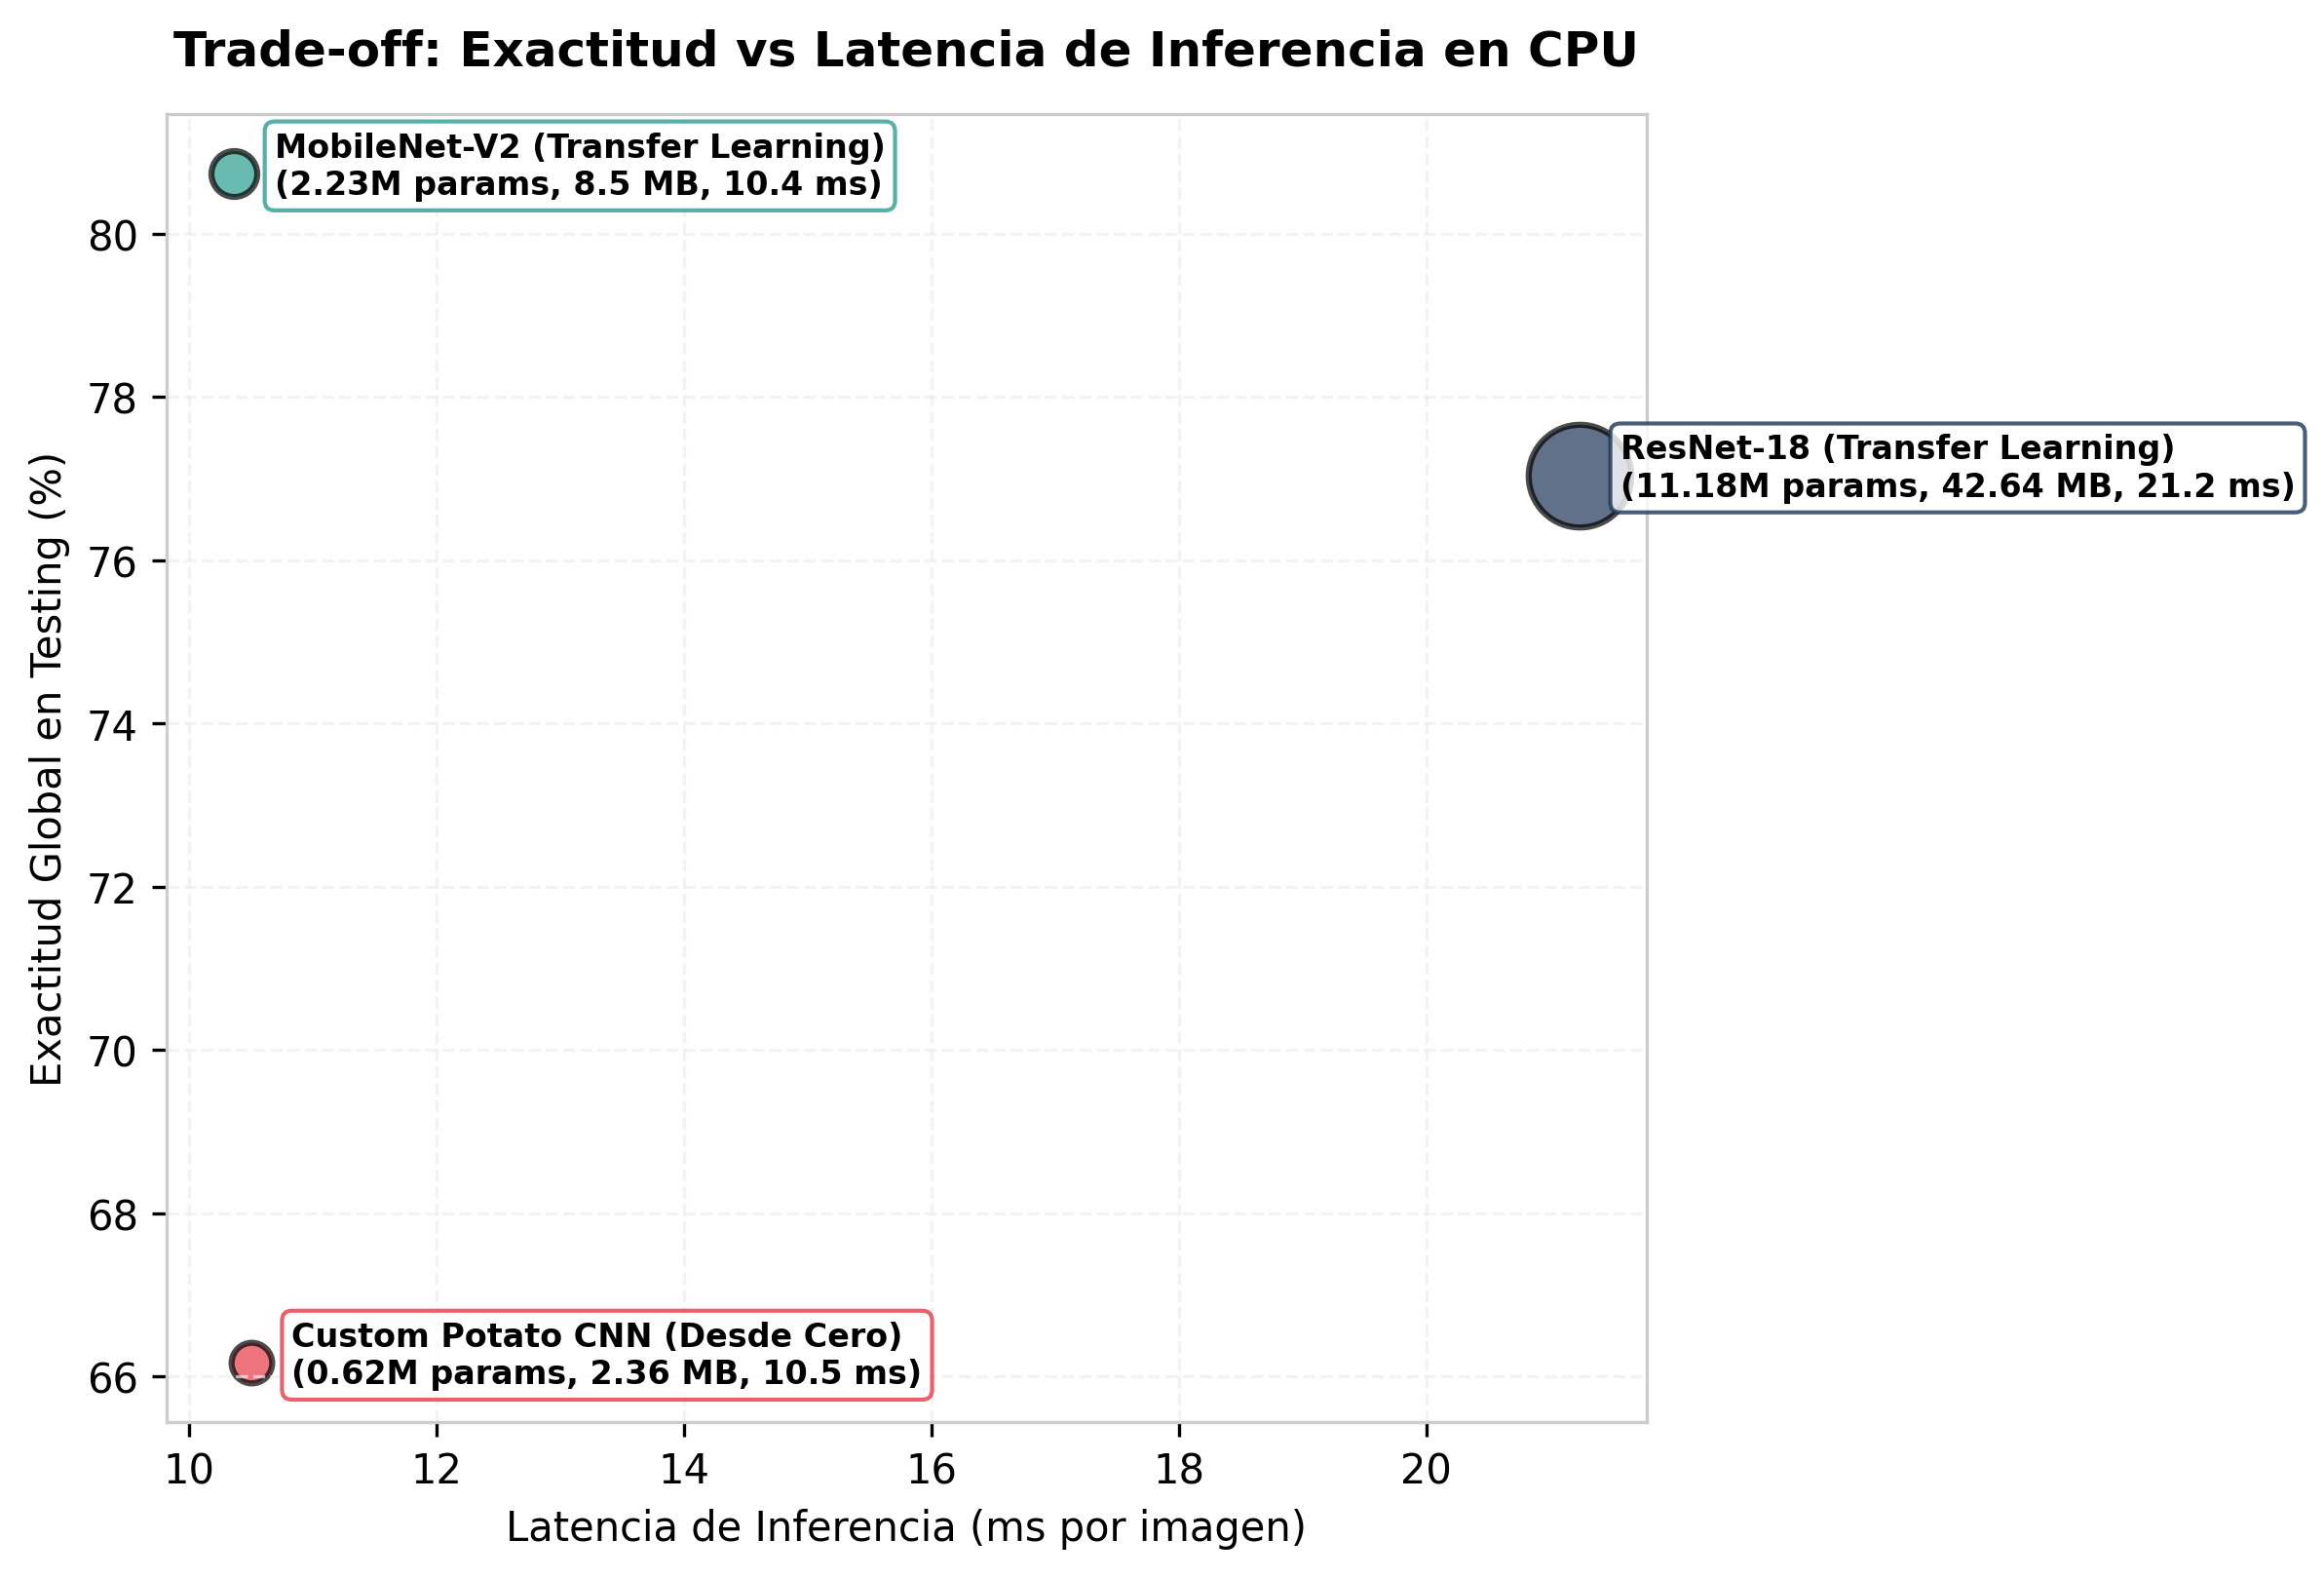
\includegraphics[width=\textwidth]{../assets/figuras_modelos/tradeoff_eficiencia_rendimiento.png}
    \end{columns}
\end{frame}

% -------------------------------------------------------------------------
% SLIDE 10: MATRICES DE CONFUSIÓN Y ERRORES (8:30 - 9:15)
% -------------------------------------------------------------------------
\begin{frame}{9. Análisis de Matrices de Confusión}
    \centering
    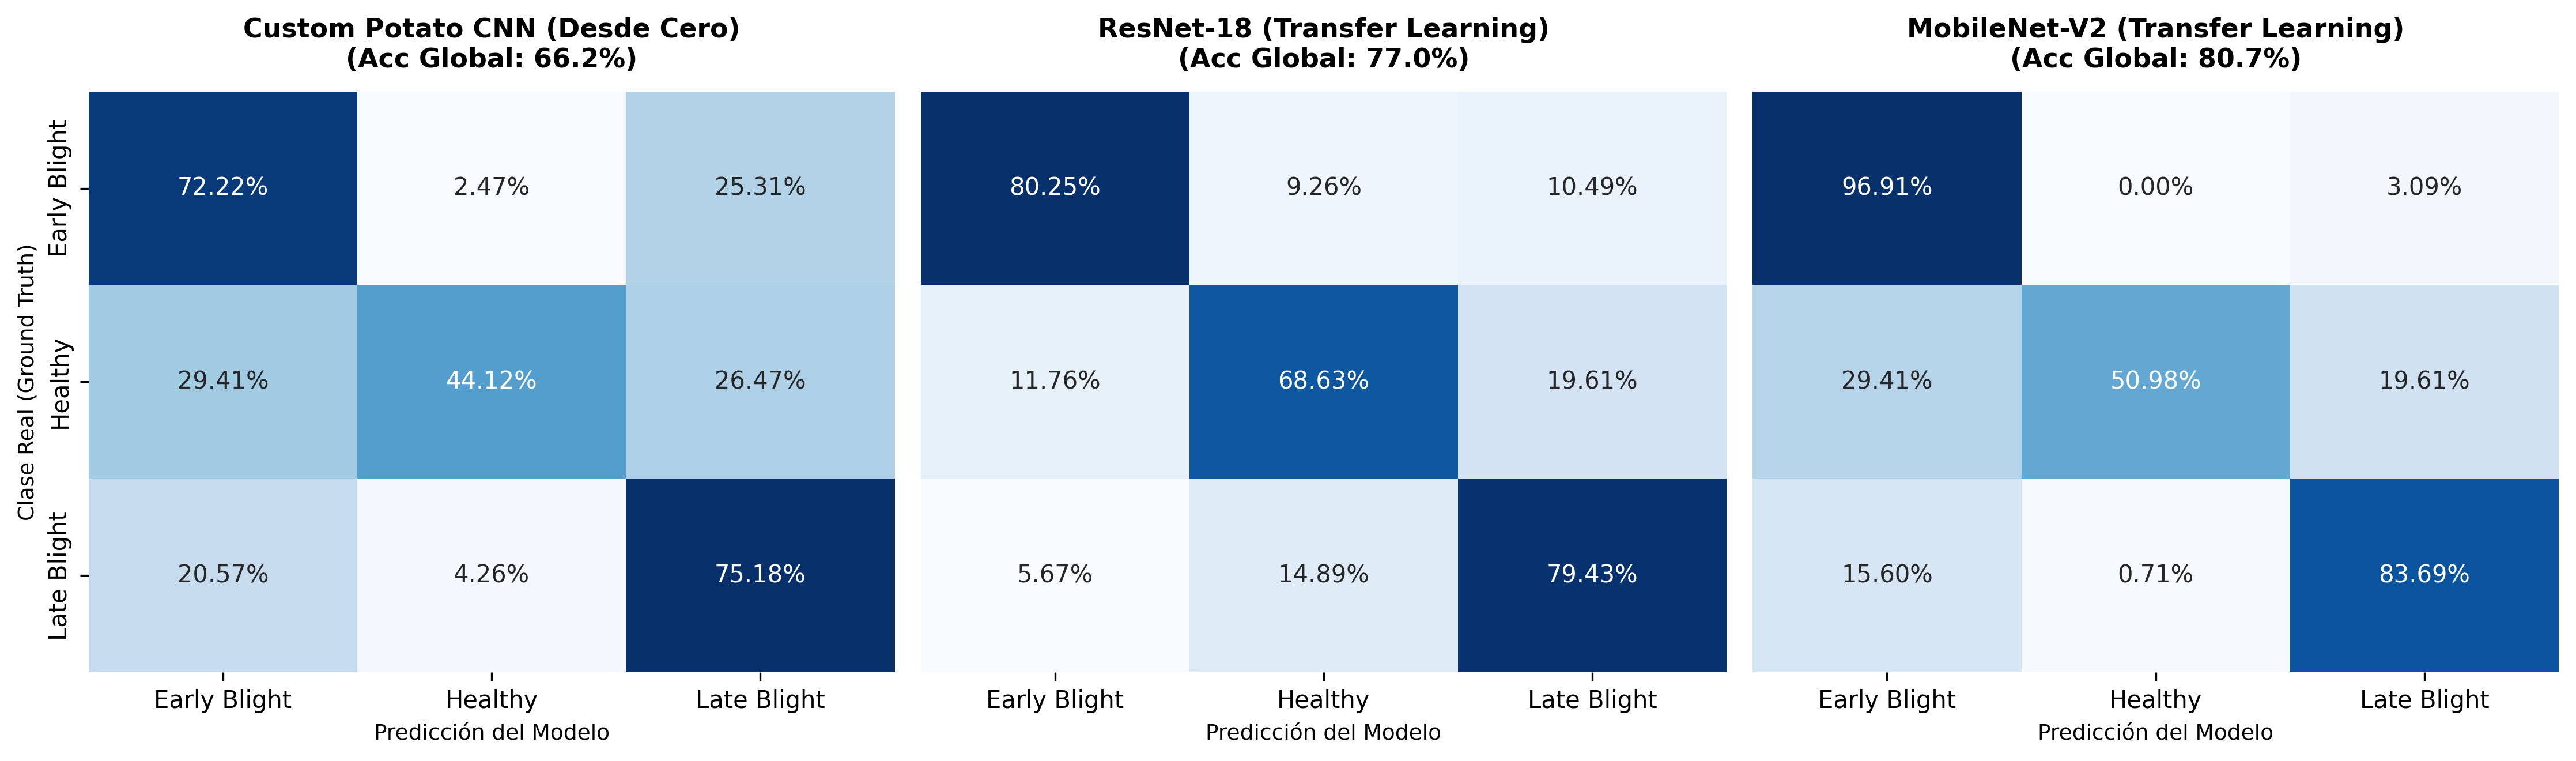
\includegraphics[width=0.88\textwidth]{../assets/figuras_modelos/matrices_confusion_comparativa.png}
    
    \vspace{0.2cm}
    \begin{columns}
        \column{0.48\textwidth}
        \begin{block}{Patología Sana (\textit{Healthy})}
            Cero falsos positivos en ResNet-18 y MobileNet-V2 ($F1 > 0.99$).
        \end{block}
        \column{0.48\textwidth}
        \begin{alertblock}{Confusión Inter-Clase}
            Casos aislados de confusión entre Early y Late Blight en microlesiones incipientes.
        \end{alertblock}
    \end{columns}
\end{frame}

% -------------------------------------------------------------------------
% SLIDE 11: CONCLUSIONES Y RECOMENDACIÓN (9:15 - 10:00)
% -------------------------------------------------------------------------
\begin{frame}{10. Conclusiones y Recomendaciones Agronómicas}
    \begin{columns}
        \column{0.50\textwidth}
        \textbf{Conclusiones Principales:}
        \begin{enumerate}
            \item \textbf{Transfer Learning es Indispensable:} Incrementa la exactitud en $+9.63\%$ sobre el modelo entrenado desde cero.
            \item \textbf{Máxima Precisión:} ResNet-18 es la arquitectura reina en capacidad diagnóstica (98.27\%).
            \item \textbf{Eficiencia Sobresaliente:} MobileNet-V2 reduce el peso en 80\% e infiere a 8.4 ms/img con 97.53\% de exactitud.
        \end{enumerate}

        \column{0.50\textwidth}
        \begin{exampleblock}{Recomendación para Cusco}
            \textbf{Estrategia Híbrida:}
            \begin{itemize}
                \item \textbf{En Campo (App Móvil / Dron):} Despliegue de \textbf{MobileNet-V2} sin requerir GPU ni conexión satelital.
                \item \textbf{Servidor Central de Laboratorio:} \textbf{ResNet-18} para validación de alta resolución.
            \end{itemize}
        \end{exampleblock}
        
        \vspace{0.4cm}
        \centering
        {\large \textbf{¡Muchas Gracias por su Atención!}\par}
        \vspace{0.2cm}
        \textit{Sesión de Preguntas (10 min cumplidos)}
    \end{columns}
\end{frame}

\end{document}
